%!TEX program = xelatex
\documentclass[10pt]{article}
\usepackage{amssymb}
\usepackage{amsmath}
\usepackage{mathrsfs}
\usepackage{titlesec}
\usepackage{xcolor}
%\usepackage[shortlabels]{enumitem}
\usepackage{enumerate}
\usepackage{bm}
\usepackage{tikz}
\usepackage{listings}
\usetikzlibrary{arrows}
\usepackage{subfigure}
\usepackage{graphicx,booktabs,multirow}
\usepackage[a4paper]{geometry}
\usepackage{upquote}
\usepackage{float}
\usepackage{pdfpages}

\usepackage[colorlinks,linkcolor=blue]{hyperref}
\usepackage{mdframed}

\iffalse
\usepackage{lastpage}
\usepackage{fancyhdr}
\fancyfoot[C]{Page \thepage\ of \pageref{LastPage}}
% Uncomment to remove the header rule
\renewcommand{\headrulewidth}{0pt} 
\pagestyle{fancy}
\fi

\geometry{verbose,tmargin=2cm,bmargin=2cm,lmargin=2cm,rmargin=2cm}
\geometry{verbose,tmargin=2cm,bmargin=2cm,lmargin=2cm,rmargin=2cm}
\lstset{language=Matlab}
\lstset{breaklines}

\input defs.tex

\newenvironment{solution}
    { \begin{mdframed}[backgroundcolor=gray!10] \textcolor{cyan}{\textbf{Solution}} \\}
    {  \end{mdframed}}

\newtheorem{proposition}{Proposition}
\newtheorem{remark}{Remark}

\titleformat*{\section}{\centering\LARGE\scshape}
\renewcommand{\thesection}{\Roman{section}}
\lstset{language=Matlab,tabsize=4,frame=shadowbox,basicstyle=\footnotesize,
keywordstyle=\color{blue!90}\bfseries,breaklines=true,commentstyle=\color[RGB]{50,50,50},stringstyle=\ttfamily,numbers=left,numberstyle=\tiny,
  numberstyle={\color[RGB]{192,92,92}\tiny},backgroundcolor=\color[RGB]{245,245,244},inputpath=code}

\begin{document}

\title{CS150: Database and Data Mining \\%
	Final Exam Solutions}
\maketitle


\section{Basics \textbf{[10 points]}}
For each image on the next page, select the letter corresponding to the best description. \\
A. Left Deep Tree \\
B. Key Compression \\
C. B+ Tree \\
D. ISAM \\
E. Nested Loops Join \\
F. Sort Merge Join \\
G. Indexed Nested Loop Join \\
H. Slotted Page \\
I. Variable Length Tuple \\
J. Fixed Length Tuple \\
K. Buffer Frame \\
L. Sort based group by \\
M. mapPartitions \\
N. Tournament Sort \\
\begin{solution}
	1. C (not an ISAM because pages non-sequential and prev/next pointers present) \\
	2. B (only prefixes are needed to search tree) \\
	3. E (a nested loops join goes through every possible pair of tuples) \\
	4. A (in fact, this is a join plan) \\
	5. H (there is a slot header holding pointers to records) \\
	6. F (this requires sorting, and it also yields pairs of records between two relations) \\
	7. I (the pointers at the record header point to the end of variable-length strings)
\end{solution}
%\newpage
\begin{figure}
	\centering
	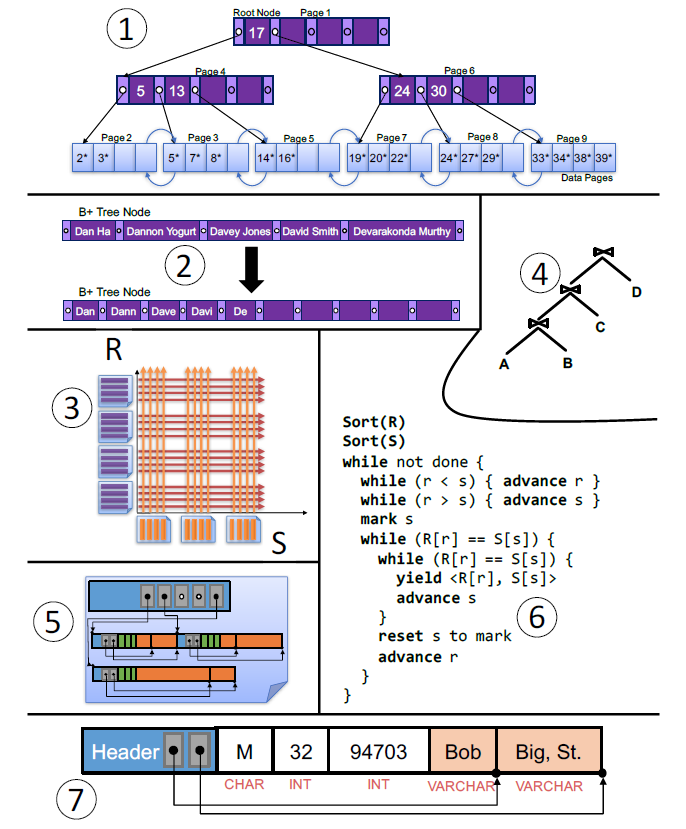
\includegraphics[width=.9\linewidth]{basics.png}
\end{figure}


\newpage
\section{SQL and ER Modeling \textbf{[12 points]}}
\begin{enumerate}

	\item \textbf{[2 points]}
	      Which of the following expressions computes the matrix vector product:
	      $$
		      (\mathbf{A} \mathbf{x})_{i}=\sum_{k=1}^{d} A_{i k} x_{k}
	      $$
	      Assume $\mathbf{A}$ and $\mathbf{x}$ have compatible dimensions and there is only one correct answer.\\
	      A.
	      \begin{lstlisting}
SELECT A.row AS row, A.value * x.value AS value 
FROM A JOIN x
ON A.row = x.row
\end{lstlisting}
	      B.
	      \begin{lstlisting}
SELECT A.row AS row, SUM(A.value * x.value) AS value 
FROM A JOIN x
ON A.row = x.row
GROUP BY A.col
\end{lstlisting}
	      C.
	      \begin{lstlisting} 
SELECT x.row AS row, SUM(A.value * x.value) AS value 
FROM A JOIN x
ON A.col = x.row
GROUP BY A.col
\end{lstlisting}
	      D.
	      \begin{lstlisting} 
SELECT A.row AS row, SUM(A.value * x.value) AS value 
FROM A JOIN x
ON A.col = x.row
GROUP BY A.row
\end{lstlisting}
	      \begin{solution}
		      D: The final answer should be grouped by the row of A and therefore sum over the product along the columns.
	      \end{solution}



	\item \textbf{[2 points]}
	      Suppose we wanted to compute the element-wise sum of the vectors $\mathbf{x}$
	      and $\mathbf{y}$ using the SQL expression:
	      \begin{lstlisting}
SELECT x.row AS row, SUM(x.value + y.value) AS value 
FROM x JOIN y 
ON x.row = y.row
\end{lstlisting}
	      Which of the following statements about this query are true?
	      (You may mark zero ($\phi$), one or more than one of the choices.)\\
	      A. Some non-zero entries may be omitted from the final result.\\
	      B. The correct query should use LEFT OUTER JOIN.\\
	      C. The correct query should use FULL OUTER JOIN.\\
	      D. There is nothing wrong.
	      \begin{solution}
		      A, C: There was a typo in this question (sum should be removed).
		      The issue with this query is the combination of two factors.
		      First, the two vectors may have zeros in different places,
		      and in a sparse vector the zero entries are represented by
		      the absence of information (missing row IDs in the table).
		      Second, by default, joins in SQL will discard a tuple from one
		      table unless it has a match in the other table; OUTER JOINs
		      preserve these non-matching tuples. \\
		      Consider the following:
		      \begin{center}
			      \begin{tabular}{|l|l|}
				      \multicolumn{2}{c} {Vector a} \\
				      \hline Row & Value            \\
				      \hline 1   & 3.0              \\
				      \hline 3   & 4.0              \\
				      \hline
			      \end{tabular} \qquad \qquad
			      \begin{tabular}{|l|l|}
				      \multicolumn{2}{c} {Vector b} \\
				      \hline Row & Value            \\
				      \hline 2   & 2.0              \\
				      \hline 5   & 8.0              \\
				      \hline
			      \end{tabular}
		      \end{center}
		      These two tables produce no outputs on a typical (inner) join,
		      representing a vector of all 0’s.  We need to do a full outer join
		      to ensure that we get rows 1, 2, 3 and 5 in the output.
	      \end{solution}

	\item \textbf{[8 points]}
	      There are four tables. SALESPERSON contains the names, ids \& quotas for the salespeople, and names are not unique.
	      PRODUCTS contains the product names, product ids, and prices for the products.
	      The product ids are unique.
	      CUSTOMERS contains the customer names, customer ids, and regions for the customers (customer ids are unique),
	      and ORDERS contains the customer id, the product id, and the product ordered per customer.\\
	      \begin{center}
		      \begin{tabular}{|l|l|l|}
			      \multicolumn{2}{c} { SALESPERSON }     \\
			      \hline Sname          & Sid & Quota    \\
			      \hline Frances        & 25  & $\$ 100$ \\
			      \hline $\mathrm{Bob}$ & 31  & $\$ 150$ \\
			      \hline Frances        & 74  & $\$ 200$ \\
			      \hline Mary           & 89  & $\$ 250$ \\
			      \hline
		      \end{tabular} \qquad
		      \begin{tabular}{|l|l|l|}
			      \multicolumn{2}{c} { PRODUCTS }  \\
			      \hline Pname    & Pid & Pprice   \\
			      \hline disks    & 131 & $\$ 100$ \\
			      \hline pcs      & 152 & $\$ 700$ \\
			      \hline macs     & 831 & $\$ 800$ \\
			      \hline printers & 255 & $\$ 120$ \\
			      \hline paper    & 221 & $\$ 5$   \\
			      \hline
		      \end{tabular} \\
		      \begin{tabular}{|l|l|l|}
			      \multicolumn{2}{l} { CUSTOMERS } \\
			      \hline Cname  & Cid & Region     \\
			      \hline Bob    & 1   & TX         \\
			      \hline Harry  & 2   & TX         \\
			      \hline Lin    & 3   & MA         \\
			      \hline Martha & 4   & FL         \\
			      \hline Lin    & 5   & FL         \\
			      \hline Leyla  & 6   & CA         \\
			      \hline
		      \end{tabular} \qquad
		      \begin{tabular}{|l|l|l|}
			      \multicolumn{3}{c} { ORDERS } \\
			      \hline Cid & Pid & Quantity   \\
			      \hline 1   & 152 & 1          \\
			      \hline 2   & 152 & 1          \\
			      \hline 4   & 831 & 1          \\
			      \hline 4   & 131 & 1          \\
			      \hline 5   & 255 & 1          \\
			      \hline 6   & 831 & 1          \\
			      \hline
		      \end{tabular}
	      \end{center}
	      \begin{itemize}
		      \item[(a)] \textbf{[2 points]} Select the true SQL expression(s) for “List the names of the customers who have bought more than one item.”
		            (You may mark zero ($\phi$), one or more than one of the choices.)\\
		            A.\begin{lstlisting}
	SELECT cname
	FROM customers
	WHERE cid IN (SELECT cid
	              FROM orders
	              GROUP BY cid
	              HAVING count(*) > 1)
\end{lstlisting}
		            B.\begin{lstlisting}
	SELECT c.cname
	FROM customers c, (SELECT cid  
	                   FROM orders
	                   GROUP BY cid
	                   HAVING count(*) > 1) as o
	WHERE c.cid = o.cid
\end{lstlisting}
		            C. \begin{lstlisting}
	SELECT cname
	FROM customers
	WHERE (SELECT count(*)
	       FROM orders
	       GROUP BY pid) > 1
\end{lstlisting}
		            D. \begin{lstlisting}
	SELECT cname
	FROM customers c, orders o1, orders o2
	WHERE c.cid = o1.cid and c.cid = o2.cid and o1.cid < > o2.pid
\end{lstlisting}
		            \begin{solution}
			            A, B: In C, ``group by pid'' is wrong.
		            \end{solution}

		      \item[(b)] \textbf{[2 points]} Select the true SQL expressions for “List the names, pid, and price of all the products, whether or not the product has been ordered,
		            but if it has been ordered by the cids of the customer who ordered it.”
		            (You may mark zero ($\phi$), one or more than one of the choices.)\\
		            A. \begin{lstlisting}
	SELECT name, pid, price, cid
	FROM products LEFT OUTER JOIN orders
\end{lstlisting}
		            B. \begin{lstlisting}
	SELECT name, pid, price, cid 
	FROM products LEFT OUTER JOIN orders
	ON products.pid = orders.pid
\end{lstlisting}
		            C. \begin{lstlisting}
	SELECT name, p.pid, price, cid
	FROM products p, orders o
	WHERE p.pid = o.pid
	UNION
	SELECT name, pid, price
	FROM products p
	WHERE NOT EXISTS (SELECT * FROM orders o WHERE o.pid = p.pid)
\end{lstlisting}
		            D. \begin{lstlisting}
	SELECT name, p.pid, price, cid
	FROM products p, orders o
	WHERE p.pid = o.pid
	UNION
	SELECT name, pid, price, NULL as cid
	FROM products p
\end{lstlisting}
		            \begin{solution}
			            A, B: In C, should be ``SELECT name, pid, price ,NULL as cid'';
						In D, should add ``WHERE NOT EXISTS (SELECT * FROM orders o WHERE o.pid = p.pid)''. \\
						We also accept $\phi$, because none of the four tables has the field ``name''.
		            \end{solution}

		      \item[(c)] \textbf{[4 points]}
		            Now, let's complete the ER diagram with the tables given above and some new translations.
		            You need to underline the primary keys, add arrows. If bolding a line/arrow,
		            be sure to clearly make it bold. If here's weak entity, also be sure to clearly show it.\\
		            •	Each product sold by exactly one salesperson.\\
		            •	The sid of salesperson in the same shop is unique, however two salesperson in different shop might have the same sid.\\
		            •	A salesperson can only work in one shop.\\
		            •	The address can uniquely identify a shop.\\
		            \begin{figure}[ht]
			            \centering
			            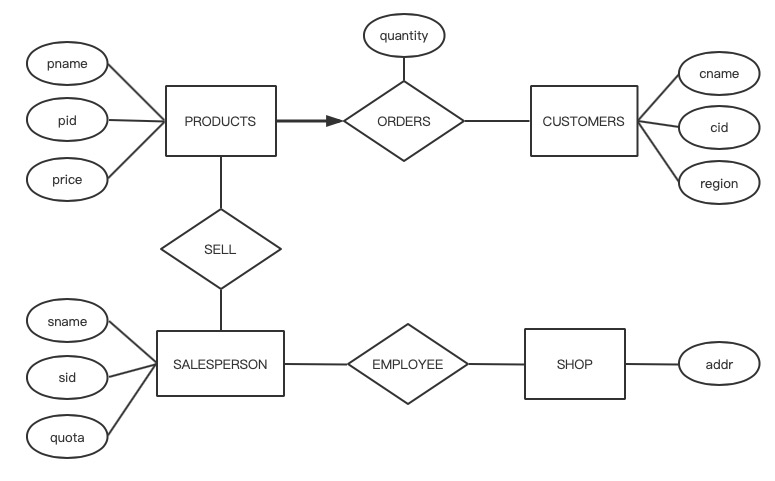
\includegraphics[width=0.7\linewidth]{E_R}
		            \end{figure}
		            \begin{solution}
			            2 bold arrow \& 1 blod entity \& 1 blod relation.
			            \begin{center}
				            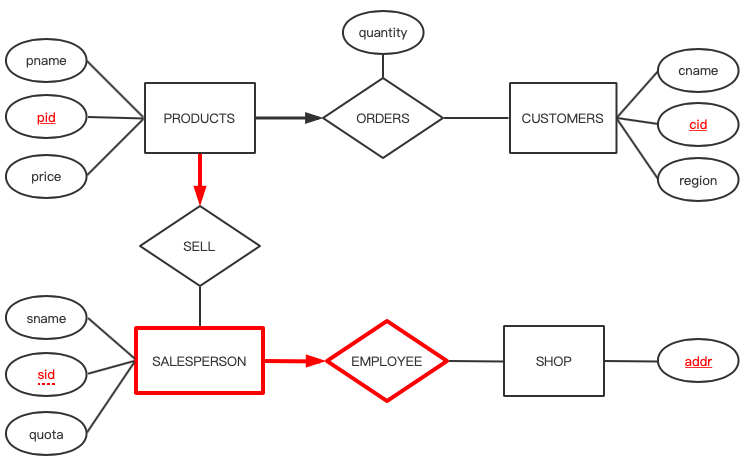
\includegraphics[width=0.8\linewidth]{ER_solution.png}
			            \end{center}
		            \end{solution}
	      \end{itemize}
\end{enumerate}


\newpage
\section{Indexes and B+ Trees \textbf{[9 points]}}

\begin{enumerate}

	\item \textbf{[5 points]} Basics of B+ Trees.
	      \begin{itemize}
		      \item[(a)] \textbf{[1 point]} What is the maximum fan out $F$ of an order $d$ B+ tree? %\underline{\hbox to 20mm{}}
		            \begin{solution}
			            The maximum fan out is the maximum occupancy plus one, or $2d + 1$, by definition.
		            \end{solution}

		      \item[(b)] \textbf{[2 points]}
		            Assume that each leaf can hold $F$ data entries. What is the maximum number of data entries
		            that an order $d$ B+ tree of height 5 can store? Express your answer as a function of $F$. (Note that a height 1 B+ tree only has a root node).
		            \begin{solution}
			            We are assuming that the leaf pages hold $F = 2d + 1$.
			            At height 1, the root node is a leaf node and therefore the index holds $F$. At height 2, there is a
			            root node and its children are leaf nodes. The root node has a max fan out of $F$ children and each
			            child is a leaf node that can hold max $F$ entries. Therefore the index can hold $F^2$ total entries. We are accepting $F^5, (2d + 1)^5$ and any other fifth power of fan out.
		            \end{solution}

		      \item[(c)] \textbf{[2 points]}
		            Again, assume that each leaf can hold $F$ data entries. And we have indexed a file with $1\times 10^9$ records with this
		            order $d$ B+ tree. What is the minimum number of I/Os it will take to check if a data entry exists in this tree?
		            Express your answer as a function of $F$.
		            \begin{solution}
			            $\lceil \log_F(\frac{10^9}{F})\rceil$
		            \end{solution}
	      \end{itemize}

	\item \textbf{[4 points]}
	      Consider the following B+ tree of order 2.
	      \begin{center}
		      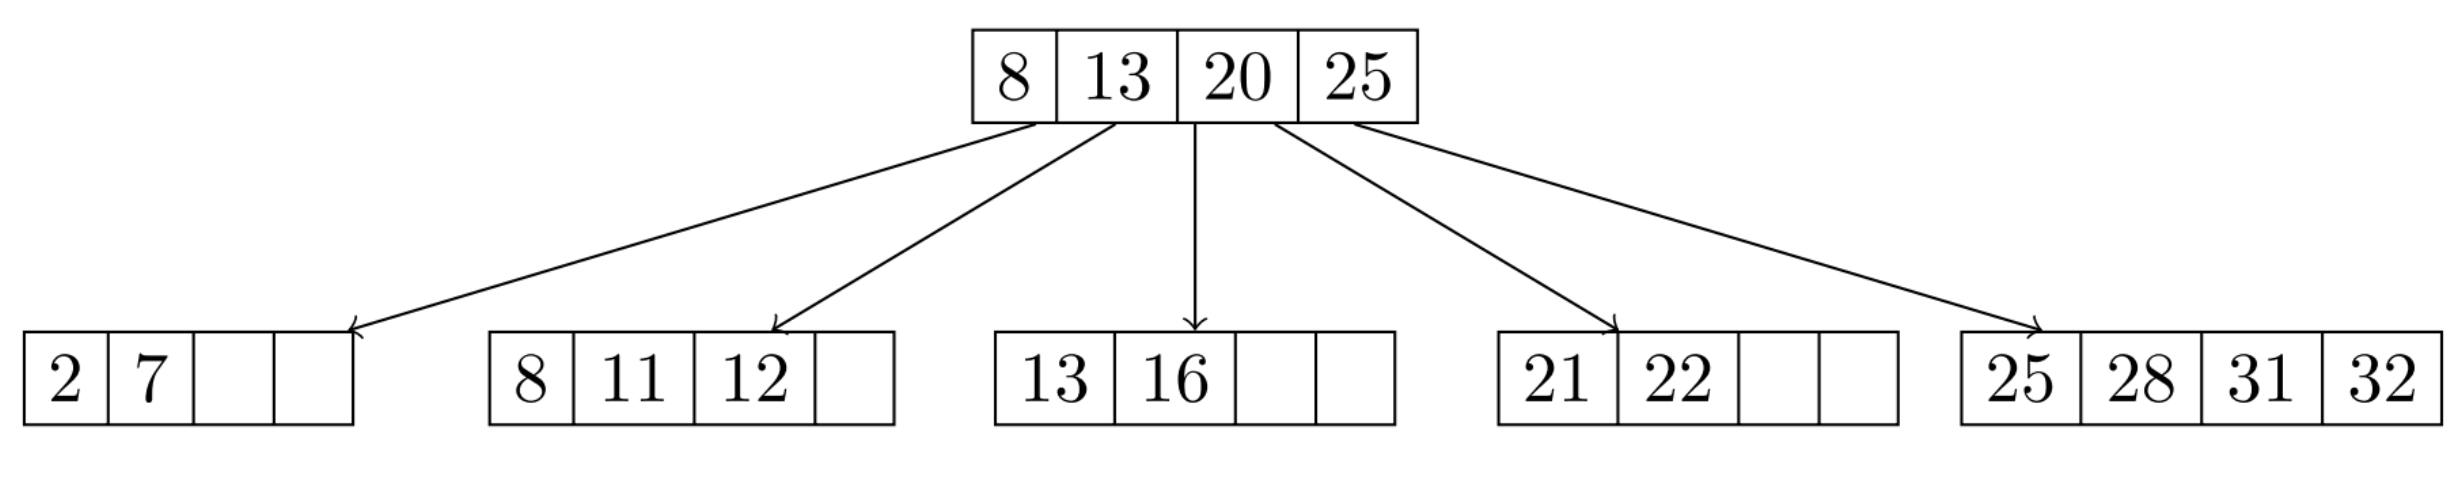
\includegraphics[scale=0.25]{Btree.png}
	      \end{center}
	      \begin{itemize}
		      \item[(a)] \textbf{[1 point]} How many nodes split when you insert 27?
		            \begin{solution}
			            \begin{itemize}
				            \item To insert 27, we follow the rightmost pointer in the tree from the root node because
				                  $27 > 8$, $27 > 13$, $27 > 20$, $27 > 25$.
				            \item We get to the leaf node containing (25, 28, 31, 32) and attempt to insert 27, but the leaf node
				                  is at maximum capacity and the insertion breaks the occupancy invariant. Therefore we must
				                  split the leaf into (25, 27) and (28, 32, 21) and copy up key 27 because this is a leaf node.
				            \item We attempt to insert 27 into the parent node containing (8, 13, 20, 25) but the root is also at
				                  maximum capacity. We split it into (8, 13) and (25, 28) pushing up key 20 because it is an
				                  inner node. Our final tree looks like and we split two nodes.
			            \end{itemize}
		            \end{solution}

		      \item[(b)] \textbf{[1 point]} After inserting 27 into the tree, you also insert 26. How many nodes split as a result of inserting
		            26?
		            \begin{solution}
			            \begin{itemize}
				            \item To insert 26, we first look at the root node and follow the right pointer because 26 $\geq$ 20. We
				                  then follow the middle pointer at the inner node below the root node because $26 > 25$ but
				                  $26 < 28$. We get to the leaf node containing (25, 27)
				            \item We attempt to insert 26 into the leaf node containing (25, 27) and since 3 is less than the
				                  occupancy invariant 4 we insert 26 and are done. We did not split any nodes.
			            \end{itemize}
		            \end{solution}

		      \item[(c)] \textbf{[2 points]} Assume that after inserting 26 and 27, you insert the keys 34, 35, 36, . . ., 100. After all these
		            insertions, what keys are in the leftmost leaf node?
		            \begin{solution}
			            You should be able to identify that we are only inserting keys into the right side of the
			            tree. This is similar to bulk loading in that the left leaf nodes will not be touched. Therefore, we
			            know that the leftmost leaf node will not be modified and will contain (2, 7) after the insertions to
			            the right side of the tree.
		            \end{solution}
	      \end{itemize}
\end{enumerate}


\newpage
\section{External Sorting \textbf{[8 points]}}
\begin{enumerate}
	\item \textbf{[2 points]} True or False:
	      \begin{itemize}
		      \item[(a)] Increasing the number of buffer pages don't affects the number of I/Os performed in Pass 0 of an external sort.
		            \begin{solution}
			            True: Regardless of the number of buffer pages,
			            every pass of an external sort (including Pass 0) performs the same number of IOs.
		            \end{solution}
		      \item[(b)] Double buffering reduces the time it takes to sort records within a single page.
		            \begin{solution}
			            False: Double buffering allows a program to concurrently perform computations
			            and fetch data from disk. Once a page of data is resident in memory,
			            double buffering will not help speed up computation on it.
		            \end{solution}
	      \end{itemize}

	\item \textbf{[6 points]}
	      Assume that each page is 4 KB large, and that you have a 24KB buffer pool (with 6 frames).
	      \begin{itemize}
		      \item[(a)] \textbf{[2 points]} How many passes would it take to externally sort an 512KB file?
		            Include the initial sorting pass and subsequent merging passes in your answer. You need to simplify your answer.
		            \begin{solution}
			            3: The file contains 128 pages, and B = 6, and thus we need
			            $\left(1+\left\lceil\log _{5}\left(\left\lceil\frac{128}{6}\right\rceil\right)\right\rceil=3\right)$ passes.
		            \end{solution}
		      \item[(b)] \textbf{[2 points]} What would be the total cost in I/Os for this external sort?
		            \begin{solution}
			            768: 2∗128∗$\#$passes = 256*3 = 768 (I/Os).
		            \end{solution}
		      \item[(c)] \textbf{[2 points]} What is the minimum number of additional buffer frames we require to reduce the number of passes
		            (from part 1) by 1?
		            \begin{solution}
			            6: In order to sort the file in two passes, we need B buffer frames
			            where $B(B - 1) \geq 128$. The smallest such B is 12.
			            Thus, the number of additional pages is 12 − 6 = 6.
		            \end{solution}
	      \end{itemize}
\end{enumerate}


\newpage
\section{Join Algorithms \textbf{[8 points]}}

\begin{enumerate}
	\item \textbf{[5 points]}
	      Consider a relation R with attributes $(x,y)$ and a relation S with attributes $(y, z)$.
	      Column $y$ in S is a key and the set of values of $y$ in R are the same as the set of values of $y$ in S.
	      Assume that there are no indexes available and that there are 25 pages in the buffer available.
	      Table R is 1,500 pages with 50 tuples per page. Table S is 400 with 100 tuples per page.
	      Compute the I/O costs for the following joins. Assume the simplest cost model, where pages are read and written one at a time.
	      \begin{itemize}
		      \item[(a)] \textbf{[1 point]} Block nested loops join with R as the outer relation and S as the inner relation.
		            \begin{solution}
			            $|R| + \lceil |R| / B \rceil \times |S| = 1500 + \lceil 1500/25 \rceil \times 400 = 25500$  OR \\
			            $|R| + \lceil |R| / (B-1) \rceil \times |S| = 1500 + \lceil 1500/24 \rceil \times 400 = 26700$ OR \\
			            $|R| + \lceil |R| / (B-2) \rceil \times |S| = 1500 + \lceil 1500/23 \rceil \times 400 = 27900$\\
			            Since, these three equations all appears in some materials, any were acceptable.
		            \end{solution}
		      \item[(b)] \textbf{[1 point]} Block nested loops join with S as the outer relation and R as the inner relation.
		            \begin{solution}
			            12500: $|S| + \lceil |S| / B \rceil \times |R| = 400 + \lceil 400/25 \rceil \times 1500 = 24400$  OR \\
			            $|S| + \lceil |S| / (B-1) \rceil \times |R| = 400 + \lceil 400/24 \rceil \times 1500 = 25900$ OR \\
			            $|S| + \lceil |S| / (B-2) \rceil \times |R| = 400 + \lceil 400/23 \rceil \times 1500 = 27400$\\
			            Since, these three equations all appears in some materials, any were acceptable.
		            \end{solution}
		      \item[(c)] \textbf{[1 point]} Sort merge join with R as the outer relation and S as the inner relation.
		            \begin{solution}
			            $\left.\left.\left.2|\mathrm{R}|\left(1+\left\lceil\log _{\mathrm{B}-1} \mid\right\rceil \mathrm{R} \mid / \mathrm{B}\right\rceil\right\rceil\right)+2|\mathrm{~S}|\left(1+\left\lceil\log _{\mathrm{B}-1}|| \mathrm{S} \mid / \mathrm{B}\right\rceil\right\rceil\right)+|\mathrm{R}|+|\mathrm{S}|$\\
			            $=\left.\left.2(1500)\left(1+\log _{24} \lceil{1500 / 25}\right\rceil\right)+2(400)\left(1+\log _{24} \lceil{400 / 25}\right\rceil\right)+1500+400=12500$\\
			            We cannot use the cost model of 3(M+N) because we cannot sort the larger of the two relations in 2 passes.
		            \end{solution}
		      \item[(d)] \textbf{[1 point]} Sort merge join with S as the outer relation and R as the inner relation.
		            \begin{solution}
			            12500: Same as (c).
		            \end{solution}
		      \item[(e)] \textbf{[1 point]} Hash join with S as the outer relation and R as the inner relation.
		            \begin{solution}
			            5700: $3( \lceil R \rceil + \lceil S \rceil ) = 3(1500 + 400) = 5700$.
		            \end{solution}
	      \end{itemize}

	\item \textbf{[3 points]}
	      Consider a new case, i.e. B>4 pages worth of buffer space, and relations M and N of size > B.
	      Please fill the blanks below with ``always'', ``sometimes'' or ``never''.
	      \begin{itemize}
		      \item[(a)] \textbf{[1 point]} Block nested loop join is \underline{\ \ \ \ \ \ \ \ \ \ } better than page-oriented nested loop join.
		            \begin{solution}
			            Always: Block nested loop join is page-oriented on steroids, and steroids are always good.
		            \end{solution}
		      \item[(b)] \textbf{[1 point]} Sort-merge join is \underline{\ \ \ \ \ \ \ \ \ \ } better than hash-join.
		            \begin{solution}
			            Sometimes: Hash join is cooler if one relation is really small and one is very large. Sort dominates if you have lots of duplicate join keys.
		            \end{solution}
		      \item[(c)] \textbf{[1 point]} Hybrid Hash-Join is \underline{\ \ \ \ \ \ \ \ \ \ } better than block-nested loops join.
		            \begin{solution}
			            Sometimes: Nested loops works for non-equijoins and hash does not.
			            For equijoins, hash is often better since it only makes a small number of passes over each relation, whereas block nested- loops still may visit the inner relation many times. If one relation fits in memory, the two algorithms are about equivalent.
		            \end{solution}
	      \end{itemize}
\end{enumerate}

%\newpage
%\section{Buffer Manager}


\newpage
\section{Query Optimization \textbf{[10 points]}}
%\subsection{Selectivity Estimation}
Consider two relations Cat(age, weight, price) and Pocket(money), with 150 tuples and 100 tuples respectively.
We have an index on Cat.age with 15 unique integer values uniformly distributed in the range [1, 15],
an index on Cat.weight with 30 unique float values uniformly distributed in the range [2001, 5000],
an index on Cat.price with 10 unique integer values uniformly distributed in the range [11, 20],
and an index on Pocket.money with 15 unique integer values uniformly distributed in the range [11, 25]. \\
%We do not have an index on Cat.price.\\
Use selectivity estimation to estimate the number of tuples produced by the following queries.
\begin{itemize}
	\item[(a)] \textbf{[1 point]} SELECT * FROM Cat
	      \begin{solution}
		      150: Select all tuples.
	      \end{solution}
	\item[(b)] \textbf{[2 points]} SELECT * FROM Cat WHERE age $\geq$ 10
	      \begin{solution}
		      60: \\
		      Selectivity = $\frac{max - v}{max - min + 1}$ + $\frac{1}{\#\  distinct\ values}$ = $\frac{5}{15}$ + $\frac{1}{15}$ = $\frac{2}{5}$, \\
		      150$\times \frac{2}{5}$ = 60.
	      \end{solution}
	\item[(c)] \textbf{[2 points]} SELECT * FROM Cat WHERE age $\textless$ 5 AND weight $\leq$ 3000
	      \begin{solution}
		      13: \\
		      Selectivity = Sel(age $\textless$ 5) $\times$ Sel(weight $\leq$ 3000) = $\frac{4}{15} \times \left( 1- \frac{2000}{3000} \right) = \frac{4}{45}$, \\
		      150 $\times \frac{4}{45}$ = 13.333 = 13.
	      \end{solution}
	\item[(d)] \textbf{[2 points]} SELECT * FROM Cat WHERE age $\textgreater$ 10 OR price $\geq$ 15
	      \begin{solution}
		      110: \\
		      Selectivity = Sel(age $\textgreater$ 10) + Sel(price $\geq$ 15) - Sel(age $\textgreater$ 10) $\times$ Sel(price $\geq$ 15) = $\frac{5}{15} + \frac{6}{10} - \frac{5}{15} \times\frac{6}{10} = \frac{11}{15}$, \\
		      150 $\times \frac{11}{15}$ = 110.
	      \end{solution}
	\item[(e)] \textbf{[3 points]} SELECT * FROM Cat, Pocket WHERE Cat.price = Pocket.money
	      \begin{solution}
		      1000: \\
		      Selectivity = $\frac{1}{\max (10,15)}$ = $\frac{1}{15}$, \\
		      150$\times$100$\times\frac{1}{15}$ = 1000.
	      \end{solution}
\end{itemize}



\newpage
\section{Transaction and Concurrency \textbf{[10 points]}}
%\href{https://drive.google.com/file/d/1Dzza4FvIVK17h_VdYF4M-TD5f-CnIY95/view}{Link to the reference}\\
Consider the following schedule. (For each of the questions below, you may mark zero ($\phi$), one
or more than one of the choices.)
\begin{center}
	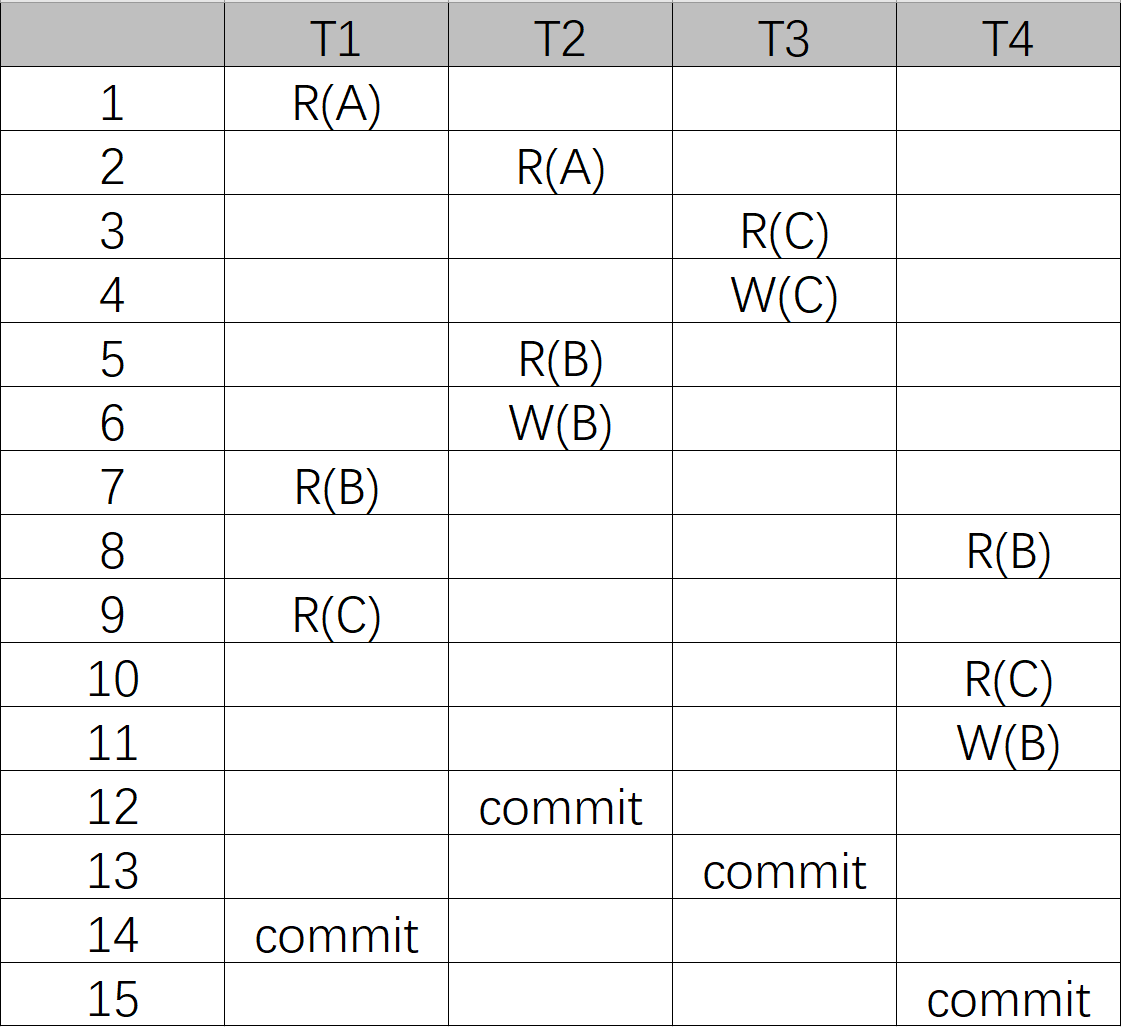
\includegraphics[scale=0.35]{transaction.png}
\end{center}
\begin{itemize}
	\item[(a)] \textbf{[1 point]} What transactions is T1 pointing to in the conflict graph for the schedule above?\\
	      A. T1\\
	      B. T2\\
	      C. T3\\
	      D. T4
	      \begin{solution}
		      D
	      \end{solution}

	\item[(b)] \textbf{[1 point]} What transactions is T2 pointing to in the conflict graph for the schedule above?\\
	      A. T1\\
	      B. T2\\
	      C. T3\\
	      D. T4
	      \begin{solution}
		      A, D
	      \end{solution}

	\item[(c)] \textbf{[1 point]} What transactions is T3 pointing to in the conflict graph for the schedule above? \\
	      A. T1\\
	      B. T2\\
	      C. T3\\
	      D. T4
	      \begin{solution}
		      A, D
	      \end{solution}

	\item[(d)] \textbf{[1 point]} What transactions is T4 pointing to in the conflict graph for the schedule above? \\
	      A. T1\\
	      B. T2\\
	      C. T3\\
	      D. T4
	      \begin{solution}
		      None
	      \end{solution}

	\item[(e)] \textbf{[3 points]} Which of the following locking disciplines could have produced the above schedule?\\
	      A. 2 phase locking\\
	      B. Strict 2 phase locking
	      \begin{solution}
		      A.\\
		      2PL is possible because each transaction could release it’s lock immediately after
		      it’s done with its operation and so this schedule would be allowed to happen. Strict 2PL is not possible because transactions have to hold their locks (ex. T1 would not be able to R(B) in 7 because T2 would have to hold its exclusive lock on B until it ends)
	      \end{solution}

	\item[(f)] \textbf{[3 points]} Which of the following schedules below are conflict equivalent to the schedule above?\\
	      A. T3, T1, T2, T4\\
	      B. T2, T3, T1, T4\\
	      C. T4, T3, T1, T2\\
	      D. T1, T2, T3, T4\\
	      E. T3, T2, T1, T4
	      \begin{solution}
		      B, E.\\
		      Just by doing a topological sort, we know that T4 has to be last and T1 has to be
		      second to last. Whether T2 or T3 comes first is irrelevant since they have no incoming edges,
		      so we have 2 possible conflict equivalent schedules.
	      \end{solution}

\end{itemize}


\newpage
\section{Logging and Recovery \textbf{[13 points]}}
\begin{enumerate}
	\item \textbf{[5 points]} \textbf{General Logging and Recovery.} \\
	      Mark the boxes for all true statement(s):
	      \begin{itemize}
		      \item[(a)] Schedules produced by two phase locking are guaranteed to prevent cascading aborts.
		            \begin{solution}
			            F: Strict 2PL is needed to guarantee this.
		            \end{solution}
		      \item[(b)] Strict two phase locking is both necessary and sufficient to guarantee conflict serializability.
		            \begin{solution}
			            F: Sufficient but not necessary.
		            \end{solution}
		      \item[(c)] In a system that uses strict two-phase locking, if a transaction aborts, it releases all of its locks as soon as rollback is complete.
		            \begin{solution}
			            T.
		            \end{solution}
		      \item[(d)] In a system that uses strict two-phase locking, a transaction that only performs reads can never enter a deadlock cycle.
		            \begin{solution}
			            F.
		            \end{solution}
		      \item[(e)] When aborting a transaction, it is necessary to modify pages on disk.
		            \begin{solution}
			            T. steal policy.
		            \end{solution}
		      \item[(f)] During recovery, the ARIES protocol redo aborted transactions.
		            \begin{solution}
			            T.
		            \end{solution}
		      \item[(g)] When a transaction commits, any modified buffer pages must be written to durable storage.
		            \begin{solution}
			            F: no force policy.
		            \end{solution}
		      \item[(h)] In ARIES recovery, after the analysis phase, the recLSN of each page in the dirty page table must be larger than the pageLSN of the corresponding page.
		            \begin{solution}
			            F: The page could have been updated and flushed from the buffer pool between the last
			            checkpoint and time of crash. The flushed page would have a pageLSN from its most recent update, which is after the recLSN in the checkpoint.
		            \end{solution}
		      \item[(i)] If PageLSN is greater than the max LSN flushed so far (flushedLSN), we can safely write this page to disk.
		            \begin{solution}
			            T: WAL requires that.
		            \end{solution}
		      \item[(j)] Write-Ahead Logging (WAL) guarantees that a transactions log records are flushed to disk before the transaction commit.
		            \begin{solution}
			            T.
		            \end{solution}
	      \end{itemize}

	\item \textbf{[8 points]} \textbf{Recovery.} \\
	      Your database server has just crashed due to a power outage.
	      You boot it back up, find the following log and checkpoint information on disk,
	      and begin the recovery process. Assume we use a STEAL/NO FORCE recovery policy.
	      \begin{figure}[h]
		      \centering
		      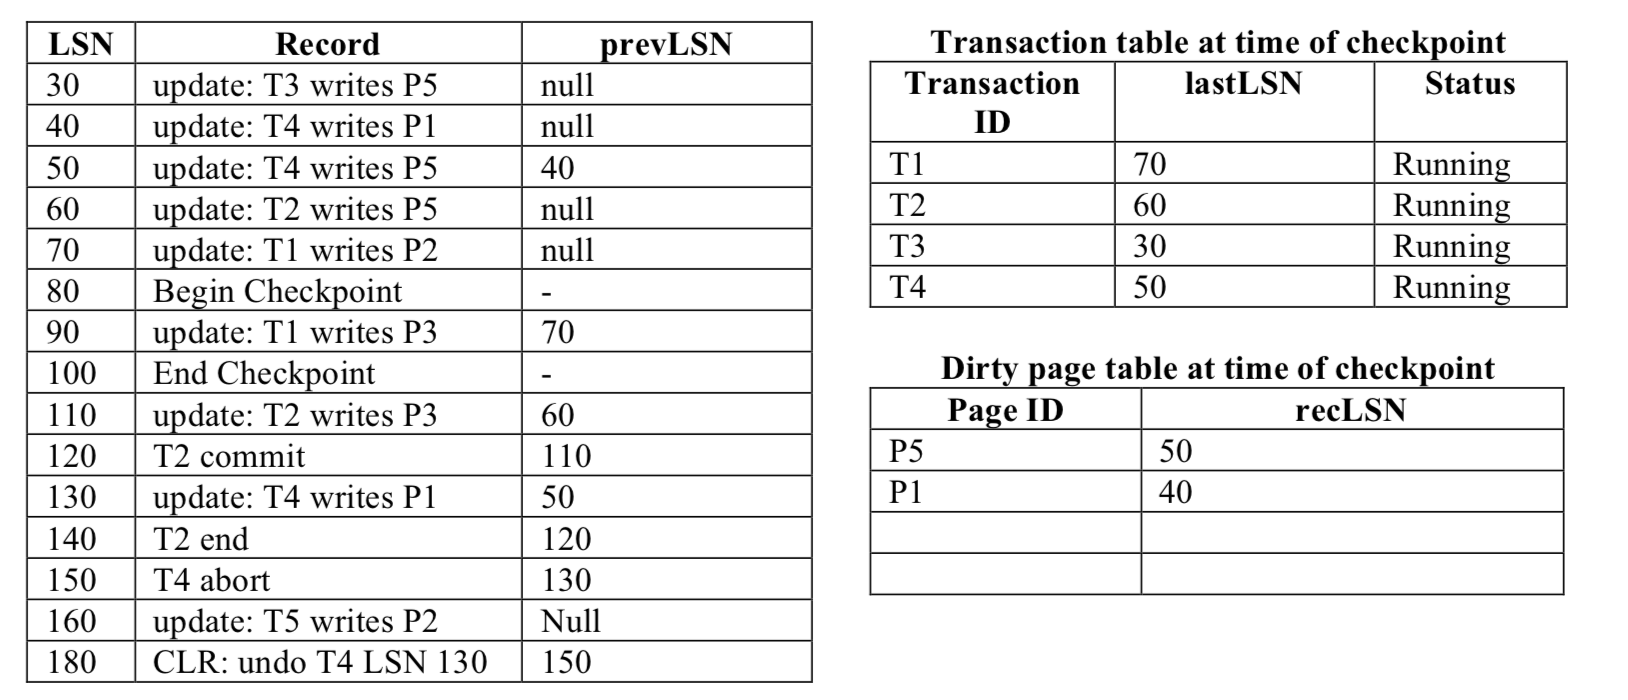
\includegraphics[width=\linewidth]{recovery}
		      %	\caption{Logging and recovery}
		      \label{fig:recovery}
	      \end{figure}
	      \begin{itemize}
		      \item[(a)] \textbf{[2 points]}
		            At the end of the Analysis phase, what transactions will be in the transaction table,
		            and with what lastLSN and Status values?
		            \begin{solution}
			            \begin{center}
				            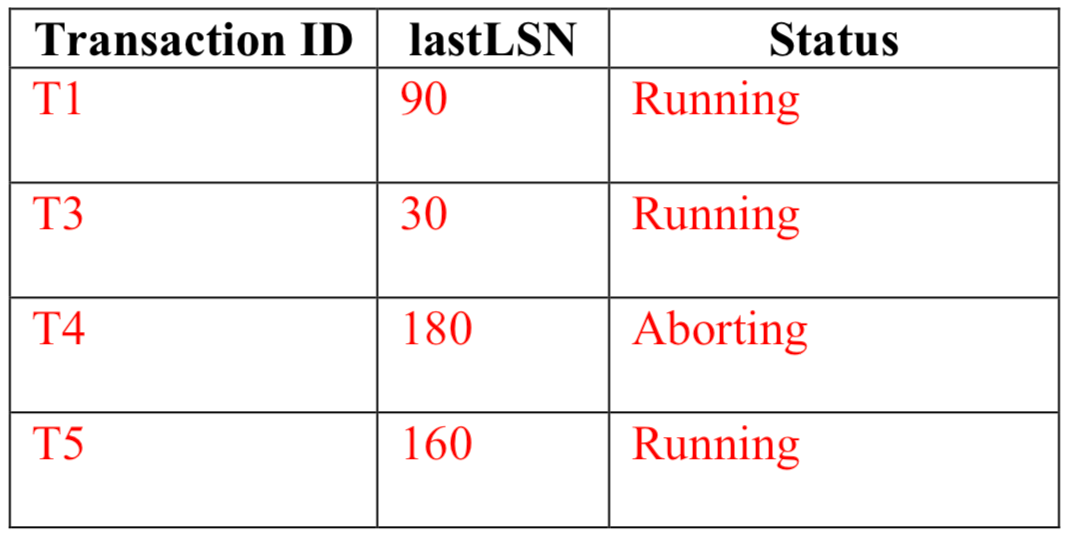
\includegraphics[width=.6\linewidth]{Xact_sol.png}
			            \end{center}
					\end{solution}
					We also accept the answer by moving the status of transactions in the above table from ``Running'' to ``Aborting''.
		      \item[(b)] \textbf{[2 points]}
		            At the end of the Analysis phase, what pages will be in the dirty page table, and with what recLSN values?
		            \begin{solution}
			            \begin{center}
				            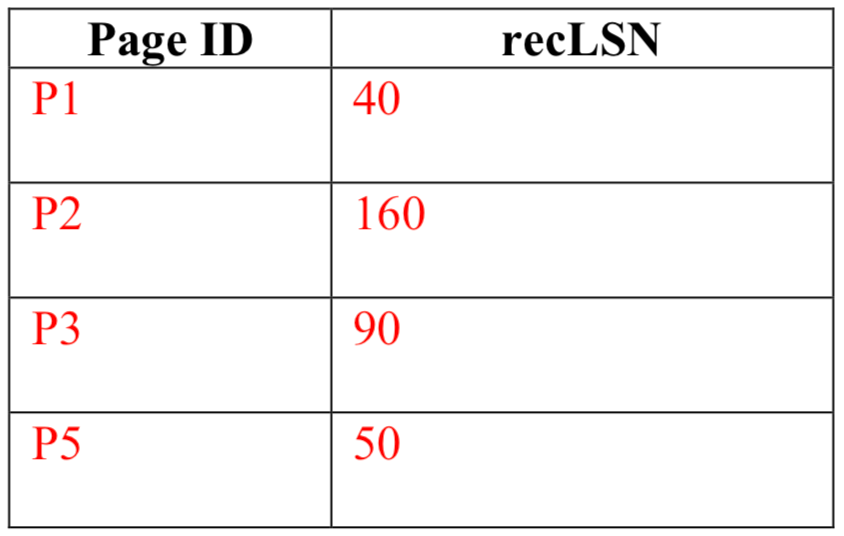
\includegraphics[width=.45\linewidth]{DPT_sol.png}
			            \end{center}
		            \end{solution}
		      \item[(c)] \textbf{[4 points]} At which LSN in the log should redo begin? Which log records will be redone (list their LSNs)?
		            \begin{solution}
			            LSN 40: Redo should begin at LSN 40, the smallest of the recLSNs in the dirty page table. \\
			            The following log records should be redone:
			            \begin{equation*}
				            40, 50, 60, 80, 90, 100, 110, 120, 130, 140, 150, 160, 180.
			            \end{equation*}
			            30 is skipped because it precedes LSN 40. 70 is skipped because P2.recLSN = 160 > 70.
			            Entries that are not updates are
			            skipped. The CLR record is not skipped, nor is the LSN that it undoes.
			            We also accept the answer:
			            \begin{equation*}
				            40, 50, 60, 90, 110, 130, 160, 180,
			            \end{equation*}
			            where only update and CLR logs are remained.
		            \end{solution}
	      \end{itemize}
\end{enumerate}


\newpage
\section{Data Mining and Machine Learning \textbf{[20 points]}}

\begin{enumerate}

	\item \textbf{[4 points]} \textbf{General Data Mining and Machine Learning.} \\
	      Mark the boxes for all true statement(s):
	      \begin{itemize}
		      \item[(a)] In multi-dimensional data model, it contains one fact table and multiple dimension tables.
		            \begin{solution}
			            True.
		            \end{solution}
		      \item[(b)] The order of the basic KDD (Knowledge Discovery in Database) process is Data Selection, Data Cleaning, Evaluation, Data Mining \& ML.
		            \begin{solution}
			            False: Data Mining comes before Evaluation.
		            \end{solution}
		      \item[(c)] In supervised machine learning labeled data is used to train a model.
		            \begin{solution}
			            True: The labeled data is the “supervision” in the name.
		            \end{solution}
		      \item[(d)] Classification models would be a good candidate when trying to predict the total
		            amount of time a user spends browsing a page.
		            \begin{solution}
			            False: Classification produces a discrete label (like “True/False”);
			            to get a numeric value like an amount of time you might want to use regression.
		            \end{solution}
		      \item[(e)] The ultimate goal in machine learning is to find a model that best fits the training data.
		            \begin{solution}
			            False: Fitting the training data is a means to the end goal of predicting unknown
			            information.  As we learned, you can overfit the training data if you make that your
			            ultimate goal.
		            \end{solution}
		      \item[(f)] The $k$-means algorithm is guaranteed to converge to the global optimum.
		            \begin{solution}
			            False: $k$-means can produce a sub-optimal answer,
			            and it sensitive to the initial position of the centers;
			            it does compute what’s called a ``local optimum''.
		            \end{solution}
		      \item[(g)] The bag-of-words model encodes text as a vector.
		            \begin{solution}
			            True.
		            \end{solution}
		      \item[(h)] A common form of feature engineering on continuous data is one-hot-encoding.
		            \begin{solution}
			            False: One-hot encoding is used for capturing the presence of boolean features.
		            \end{solution}
	      \end{itemize}

	\item \textbf{[8 points]} \textbf{K-Means.}
	      \begin{itemize}
		      \item[(a)] \textbf{[2 points]} True or False: \\
		            %A. No matter which points are selected as the initial cluster centers, the K-means algorithm is guaranteed to converge to the global optimum.\\
		            Suppose we are going to cluster the following dataset: $\{(x_1, y_1), ..., (x_n, y_n)\}$,
		            denote $\Bar{x} = \frac{1}{n}\sum_{i=1}^n x_i$ and $\Bar{y} = \frac{1}{n}\sum_{i=1}^n y_i$,
		            we can have a decentralized dataset $\{(x_1', y_1'), ..., (x_n', y_n')\}$
		            where $x_i' = x_i - \Bar{x}$, $y_i' = y_i - \Bar{y}$, $i = 1,2,...,n$.
		            The $k$-means algorithm will converge to the same result if we choose the initial
		            centers as $\{(x_s, y_s), (x_t, y_t)\}$ for the original dataset and $\{(x_s', y_s'), (x_t', y_t')\}$
		            for the decentralized dataset, where $s, t$ are two different constants.
		            \begin{solution}
			            True
		            \end{solution}

		      \item[(b)] \textbf{[2 points]}
		            Which of the following can act as possible termination conditions in $k$-means?
		            (you may mark zero ($\phi$), one or more than one of the choices.)\\
		            A. For a fixed number of iterations.\\
		            B. Assignment of observations to clusters does not change between iterations. Except for cases with a bad local minimum.\\
		            C. Centroids do not change between successive iterations.\\
		            D. Terminate when RSS falls below a threshold.
		            \begin{solution}
			            A, B, C, D.\\
			            All four conditions can be used as possible termination condition in K-Means clustering:

			            This condition limits the runtime of the clustering algorithm, but in some cases the quality of the clustering will be poor because of an insufficient number of iterations.
			            Except for cases with a bad local minimum, this produces a good clustering, but runtimes may be unacceptably long.
			            This also ensures that the algorithm has converged at the minima.
			            Terminate when RSS falls below a threshold. This criterion ensures that the clustering is of a desired quality after termination. Practically, it’s a good practice to combine it with a bound on the number of iterations to guarantee termination.
		            \end{solution}


		      \item[(c)] \textbf{[2 points]}
		            In which of the following cases will $k$-means clustering fail to give good results?
		            (you may mark zero ($\phi$), one or more than one of the choices.)\\
		            A. Data points with outliers.\\
		            B. Data points with different densities.\\
		            C. Data points with round shapes.\\
		            D. Data points with non-convex shapes.
		            \begin{solution}
			            A, B, D.\\
			            K-Means clustering algorithm fails to give good results when the data contains outliers, the density spread of data points across the data space is different and the data points follow non-convex shapes.
		            \end{solution}

		      \item[(d)] \textbf{[2 points]}
		            The following is a set of one-dimensional points: $\{-4, 0, 1, 2, 3, 5, 7, 10, 13, 22\}$, perform two iterations of $k$-means on these points using the two initial centroids 1 and 7.
		            \begin{itemize}
			            \item[1)] What are the two new centroids after the first iteration?
			            \item[2)] What are the two new centroids after the second iteration?
		            \end{itemize}
		            \begin{solution}
			            first iteration: 2/5; 57/5\\
			            second iteration: 7/6; 13
		            \end{solution}
	      \end{itemize}

	\item \textbf{[8 points]} \textbf{Linear Regression.} \\
	      Given a set of i.i.d. data points $(x_{1},y_{1})\cdots(x_{n},y_{n})$,
	      where $x \in \mathbb{R}$ and $y \in \mathbb{R}$ denote the input feature and the output response, respectively.
	      By assuming the linear model is a reasonable approximation, we consider fitting the model via least squares approaches,
	      in which we choose coefficients $\theta$ and $\theta_0$ to minimize the Residual Sum of Squares (RSS),
	      \begin{equation}
		      \hat{\theta},~ \hat{\theta}_0 = \argmin_{\theta,~ \theta_0}~ \sum_{i=1}^{n}(y_{i} -\theta x_{i}-\theta_0)^{2}.
		      \label{eq:1}
	      \end{equation}
	      Based on 5 observations of $(x, y)$:
	      \begin{equation}
		      (1,2), \quad (2,3), \quad (3,5), \quad (4,4), \quad (5,6),
	      \end{equation}
	      please answer the following questions:
	      \begin{itemize}
		      \item[(a)] \textbf{[1 point]} Draw a 6 by 6 space with all the 5 data points.
		            \begin{solution}
			            \begin{center}
				            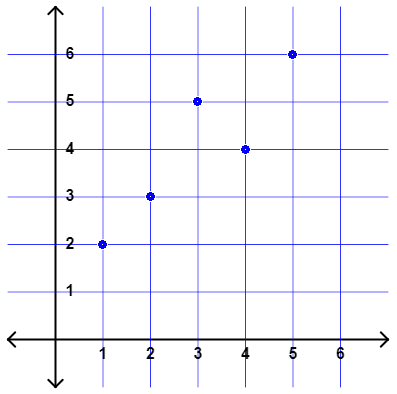
\includegraphics[width=.6\linewidth]{c_sol1.png}
			            \end{center}
		            \end{solution}
		      \item[(b)] \textbf{[3 points]} Estimate the model parameters $\theta$ and $\theta_0$.
		            \begin{solution}
			            $\hat{\theta} = \frac{9}{10}, \ \hat{\theta}_0 = \frac{13}{10}$: \\
			            By setting the derivative of the objective function w.r.t. $\theta$ and $\theta_0$ equal to 0, we have
			            \begin{align}
				            \hat{\theta}     & = \tfrac{\sum_{i=1}^{n}(x_{i}-\bar{x})(y_{i}-\bar{y})}{\sum_{i=1}^{n}(x_{i}-\bar{x})^{2}}, \\
				            \hat{\theta}_{0} & = \bar{y} -\hat{\theta}\bar{x},
			            \end{align}
			            where $\bar{x} = \tfrac{1}{n}\sum_{i=1}^{n}x_{i} = 3$ and $\bar{y} = \tfrac{1}{n}\sum_{i=1}^{n} y_{i} = 4$.
			            Then, substituting the 5 data points into the above solutions, immediately leads to our solution.
		            \end{solution}
		      \item[(c)] \textbf{[2 points]} Using~\eqref{eq:1}, argue that the least squares line,
		            \begin{equation}
			            y = \hat{\theta}x + \hat{\theta}_0,
		            \end{equation}
		            always passes through the points $(0,\hat{\theta}_0)$ and $(\bar{x},\bar{y})$,
		            where $\bar{x} = \tfrac{1}{5}\sum_{i=1}^{5}x_{i}$ and $\bar{y} = \tfrac{1}{5}\sum_{i=1}^{5} y_{i}$, and plot the line in the picture of (a).
		            \begin{solution}
			            Because $(0,\hat{\theta}_0) = (0,\frac{13}{10})$ and $(\bar{x},\bar{y})=(3,4)$ satisfy the learned least squares line $y = \frac{9}{10} x + \frac{13}{10}$.
			            Therefore, these two points determine the our line, and we can plot it in the following figure.
			            \begin{center}
				            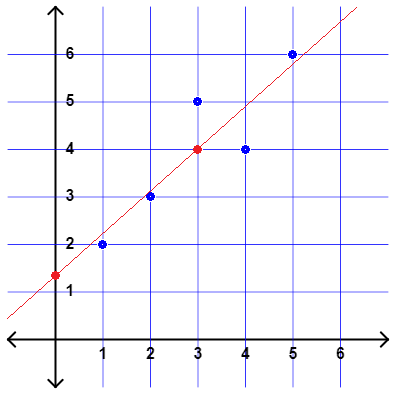
\includegraphics[width=.6\linewidth]{c_sol2.png}
			            \end{center}
		            \end{solution}
		      \item[(d)] \textbf{[2 points]} Find the data point which makes the highest contribution to RSS, and show the geometric interpretation in the picture of (a).
		            \begin{solution}
			            $(3, 5)$: \\
			            The contribution to RSS is measured by $\left( y_i - \left(\hat{\theta}x_i + \hat{\theta_0}\right) \right)^2= \left( y_i - \left(\frac{9}{10} x_i + \frac{13}{10}\right) \right)^2$,
			            and the highest contribution $\left( y_i - \left(\frac{9}{10} x_i + \frac{13}{10}\right) \right)^2 = (5-4)^2 = 1$ is made by the point $(3,5)$.\\
			            It actually indicates the area of the red square showed in the figure below.
			            \begin{center}
				            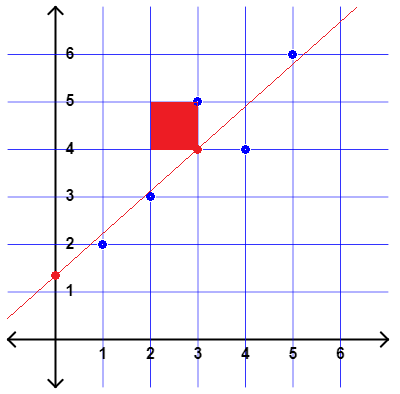
\includegraphics[width=.6\linewidth]{c_sol3.png}
			            \end{center}
		            \end{solution}
	      \end{itemize}

\end{enumerate}

\end{document}

